\subsection{Dalvik Executionable File Format} \label{subsection:android-dex}
As explained in chapter~\cite{subsection:foundation-android-package}, Android applications deliver their code in \gls{dex} bytecode and are executed by the \gls{dvm}.
The dex file format is compiled from Java bytecode. It is similar to Java bytecode except some differences.
The biggest difference is the concept how the code is executed.
While the Java \gls{vm} is stack-based the \gls{dvm} is register-based, this circumstances have influence on the code.
In addition the Dalvik bytecode is more suited to run on the ARM architecture since it supports direct mapping from dex registers to the registers of the ARM processor.
Registers in \gls{dex} bytecode are 32bits wide and store values such as integers or float values.
In case there are 64bit values, adjacent registers are used to store it.
The Java bytecode is actually more compact since it uses 8bit constants while \gls{dex} bytecode has instructions of 16bit multiples.
The \gls{dex} bytecode supports 218 valid opcodes which have a source-destination ordering for its arguments.
The arguments of the instruction refer to indexes in the pools which can be seen in figure~\ref{fig:dex}.
\newline
\begin{figure}[h]
    \centering
    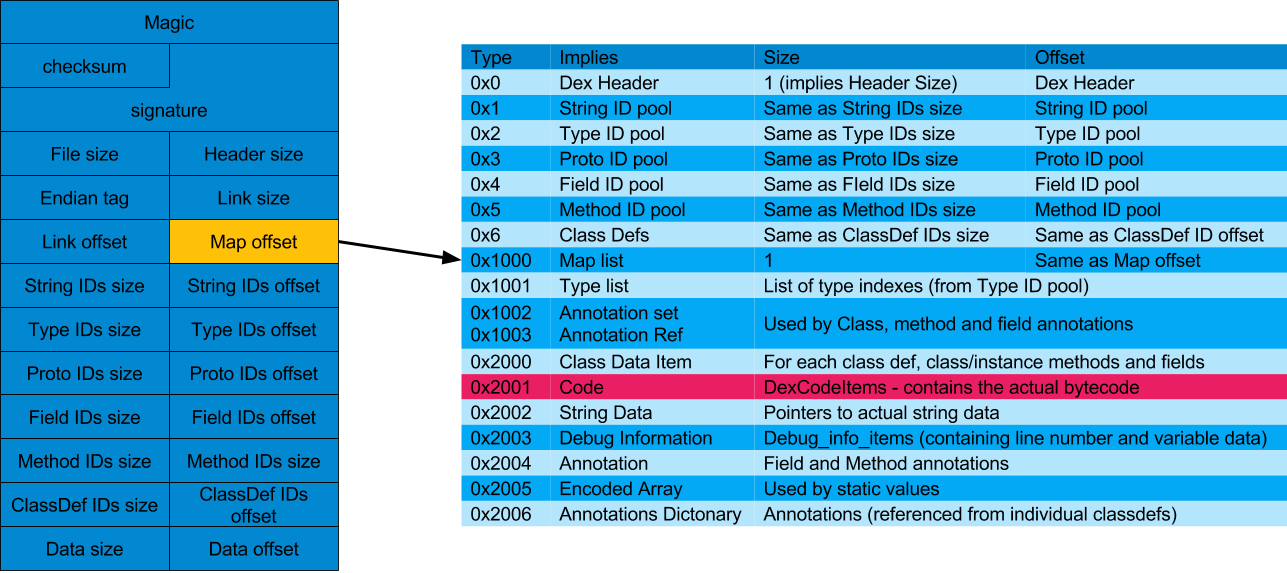
\includegraphics[width=0.8\textwidth]{data/dex.png}
    \caption{\gls{dex} file format \cite{andevconDalvikART}}
    \label{fig:dex}
\end{figure}

In order to create the dex file, dx is used on the \gls{jar} file.
Dx compiles the Java bytecode to \gls{dex} byte code and sorts string, type and method from the heterogenous pool of each class into global pools.
This results in figure~\ref{fig:dex} and figure~\ref{fig:java}.

\begin{figure}[h]
    \centering
    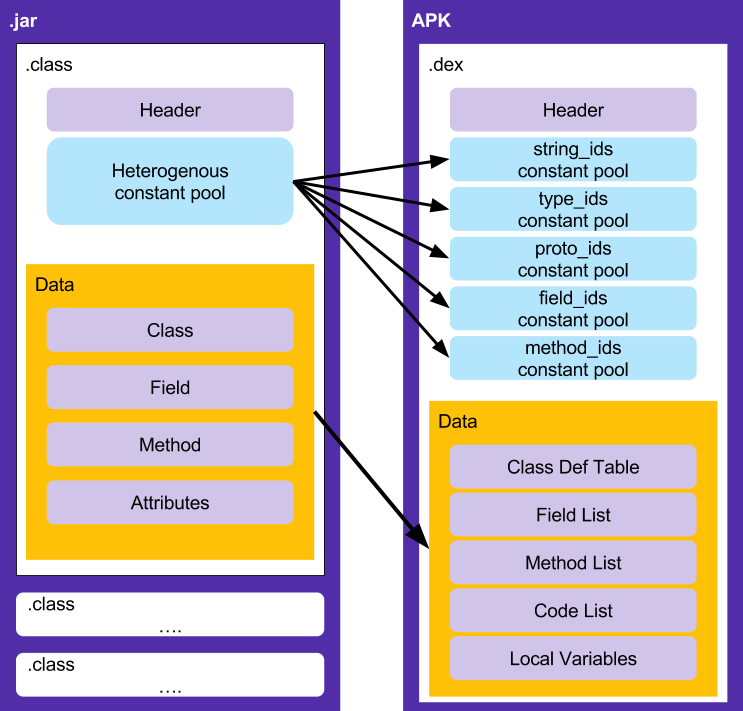
\includegraphics[width=0.5\textwidth]{data/java.png}
    \caption{\gls{jar} to \gls{apk} transformation \cite{googleDalvik}}
    \label{fig:java}
\end{figure}

When merging the resource pools, dublicates are removed.
This is most effective for string and results in a decrease of the memory footprint by up to 44\% lower in contrast to the \gls{jar}.
The result is that the \gls{dex} file has significant more references than the \gls{jar} file.
The \gls{dex} file is stored as classes.\cite{ehringerDalvik}
\newline
\newline
Since \gls{dex} bytecode supports optimization, improvements for the underlying architecture can be applied to the bytecode upon installation.
The resulting \gls{dex} file is called \gls{odex}.
The optimizations are executed by a programm called dexopt which is part of the Android plattform.
For the \gls{dvm} it makes no difference whether \gls{dex} or \gls{odex} files are executed, except speed improvements.
\newline
Bytecode has also a downside.
Like Java bytecode, \gls{dex} bytecode allows easy decompilation to Java.
Since the bytecode is, in contrast to other architectures, pretty simple to understand as well as protection is applied rarely since it has to be done by the developer itself, it is an easy target for reverse engineering.
